\section{GnuPG und Thunderbird}
Die folgende Anleitung erl�utert den Einsatz von \textbf{GnuPG} in Kombination mit  \textbf{Thunderbird}, dem E-Mail Client der Mozilla Foundation. Alle Komponenten stehen f�r Linux, Mac OS und WINDOWS kostenfrei zur Verf�gung:

\subsection{Installation von GnuPG}
GnuPG ist eine frei nutzbare Implementierung des OpenPGP Standards zur Verschl�sselung und Signierung von Daten. Es wird vom GNU Projekt st�ndig weiterentwickelt.\\

\begin{description}
 \item[Linux:] alle Distributionen installieren GnuPG standardm��ig.
 \item[MacOS:] nutzen Sie die GPGTools \footnote{ \href{http://www.gpgtools.org/}{http://www.gpgtools.org}}.
 \item[Windows 1:] Das Projekt gpg4win \footnote{ \href{http://www.gpg4win.org/}{http://www.gpg4win.org}} stellt ein Paket f�r Windows bereit mit GnuPG v. 2.0 und dem GNU Privacy Assisten f�r die Schl�sselverwaltung. 
 \item[Windows 2:] Ich kann auch das Paket GpgSX  \footnote{ \href{http://gpgsx.berlios.de/}{http://gpgsx.berlios.de}} empfehlen, welches neben GunPG einige zus�tzliche Tools enth�lt (grafische Schl�sselverwalung, Erweiterung f�r den Explorer).

\begin{figure}[htb]
\begin{center}
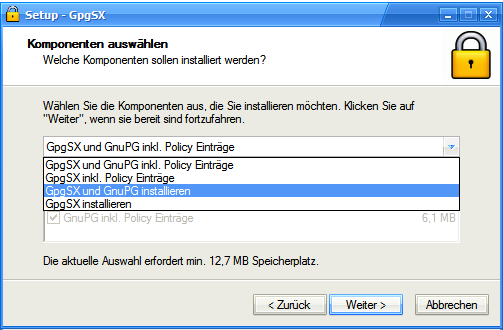
\includegraphics[scale=0.55]{../screenshots/gpgsx1.png}
\caption{GpgSX Installation}
\label{abb:gpgsx}
\end{center}
\end{figure}

 Nach dem Download ist das Setup-Programm zu starten und den Anweisungen zu folgen. Die Komponenten GnuPG und GpgSX sind zu installieren.

 \end{description}